%%%%%%%%%%%%%%%%%%%%%%%%%%%%%%%%%%%%%%%%%%%%%%%%%%%%%%%%%%%%%%%%%%%%%%%%%%%%%%%%
%2345678901234567890123456789012345678901234567890123456789012345678901234567890
%        1         2         3         4         5         6         7         8

\documentclass[letterpaper, 10 pt, conference]{ieeeconf}  % Comment this line out
                                                          % if you need a4paper
%\documentclass[a4paper, 10pt, conference]{ieeeconf}      % Use this line for a4
                                                          % paper

\IEEEoverridecommandlockouts                              % This command is only
                                                          % needed if you want to
                                                          % use the \thanks command
\overrideIEEEmargins
% See the \addtolength command later in the file to balance the column lengths
% on the last page of the document
%!TEX encoding = UTF-8 Unicode



% The following packages can be found on http:\\www.ctan.org
\usepackage{graphicx} % for pdf, bitmapped graphics files
%\usepackage{epsfig} % for postscript graphics files
%\usepackage{mathptmx} % assumes new font selection scheme installed
%\usepackage{times} % assumes new font selection scheme installed
%\usepackage{amsmath} % assumes amsmath package installed
%\usepackage{amssymb}  % assumes amsmath package installed
\usepackage{xcolor}
\usepackage[utf8]{inputenc}

% custom commands
\newcommand\todo[1]{\textcolor{red}{#1}}
\newcommand\TODO[1]{\textcolor{red}{#1}}

\title{\LARGE \bf
Homework 1 - Reperimento dell'Informazione - A.A. 18/19
}

%\author{ \parbox{3 in}{\centering Huibert Kwakernaak*
%         \thanks{*Use the $\backslash$thanks command to put information here}\\
%         Faculty of Electrical Engineering, Mathematics and Computer Science\\
%         University of Twente\\
%         7500 AE Enschede, The Netherlands\\
%         {\tt\small h.kwakernaak@autsubmit.com}}
%         \hspace*{ 0.5 in}
%         \parbox{3 in}{ \centering Pradeep Misra**
%         \thanks{**The footnote marks may be inserted manually}\\
%        Department of Electrical Engineering \\
%         Wright State University\\
%         Dayton, OH 45435, USA\\
%         {\tt\small pmisra@cs.wright.edu}}
%}

\author{Eugen Saraci - 1171697 \\ 
        Università degli Studi di Padova\\
        {\tt\small eugen.saraci@studenti.unipd.it}% <-this % stops a space
}


\begin{document}



\maketitle
\thispagestyle{empty}
\pagestyle{empty}


\section{INTRODUZIONE}
L'homework consiste nel confronto fra diverse configurazioni di un sistema di reperimento differenziati principalmente dal modello di retrieval e dalle diverse pipeline di preprocessing utilizzati. Il corpus dei documenti è rappresentato dalle collezioni sperimentali Disks4\&5 di TREC7, consistenti in circa 528.000 documenti di cui abbiamo a disposizione 50 topic con giudizi di rilevanza binari. L'obiettivo è quindi utilizzare un qualsiasi sistema di reperimento citato a lezione ed analizzare le performance delle varie configurazioni richieste, determinando, ad esempio, quale sia la migliore.
\noindent
Le varie configurazioni (che chiamerò per semplicità \textit{sistemi\footnote{Con sistema intendo la coppia composta dal modello di reperimento e dalla pipeline. Da non confondere con la parola sistema intesa ad indicare Terrier nel suo complesso.}} nel proseguo) sono le seguenti:

\begin{table}[h]
\centering
\begin{tabular}{|l|l|l|}
\hline
\textbf{Model} & \textbf{Pipeline steps}        & \textbf{Short name} \\ \hline
BM25                            & PorterStemmer, Stopwords & \texttt{bm25\_full}          \\ 
TF IDF                          & PorterStemmer, Stopwords & \texttt{tf\_idf\_full}       \\ 
BM25                            & PorterStemmer            & \texttt{bm25\_nostop}        \\
TF IDF                          & --                       & \texttt{tf\_idf\_none}       \\ \hline 
\end{tabular}
\caption{Le quattro configurazioni richieste dall'homework. La colonna ``short name'' contiene i nomi con cui si farà riferimento ai singoli sistemi.}
\label{tab:systems}
\end{table}

Il sistema di reperimento che ho deciso di utilizzare per l'homework è Terrier (ver. 4.4), mentre la libreria utilizzata per l'evaluation è \texttt{trec\_eval};\todo{link a terrier e trec eval} per i test statistici sono stati utilizzati i moduli Python \texttt{scipy.stats}\cite{scipy} e \texttt{statsmodels}\cite{statsmodels}.

\subsection{Organizzazione della relazione}
Nella Sezione \ref{sec:sw} presento brevemente il software siluppato; nella Sezione \ref{secsec:} fornisco una descrizione di quelli che sono stati i passaggi fondamentali che hanno portato al completamento dell'homework.

\section{SOFTWARE SVILUPPATO}\label{sec:sw}

Terrier offre una ampia possibilità di scripting, per tale motivo ho deciso di sviluppare degli script in Bash e Python al fine di automatizzare il processo che va dal preprocessing iniziale dei documenti fino alla stampa dei plot dei test statistici, coprendo tutti i passaggi richiesti dall'homework.
Il software sviluppato, seppur commentato e documentato con cura, non è orientato al riuso, è bensì un modo veloce che permette di replicare con semplicità i risultati ottenuti.
L'utente interessato alla replicazione dei risultati deve solamente scaricare il corpus dei documenti (ovvero la cartella TIPSTER), spostarla all'interno delle cartelle del progetto come specificato nelle istruzioni, e solo a quel punto dovrà eseguire lo script denominato \texttt{main.sh}.

La documentazione completa (in inglese), le istruzioni per l'utilizzo, ed il software stesso sono reperibili alla repository presente al link \texttt{https://github.com/esaraci/IR-HW1} resa pubblica in data: \todo{aggiungere data}. Nella repository sono presenti anche tutte le tabelle e le immagini generate dagli script, molte delle quali non sono riportate in questo elaborato.

\section{FASI OPERATIVE}\label{sec:devops}
L'homework è suddivisibile, secondo personale interpretazione, in cinque fasi distinte:
\begin{enumerate}
\item Preprocessing;
\item Indexing;
\item Retrieval;
\item Evaluation;
\item Hypothesis Testing;
\end{enumerate}
Le fasi (2), (3), e (4) sono effettuate per ognuno dei quattro sistemi elencati in Tabella \ref{tab:systems}; la fase (1) è relativa alla preparazione dei file; la fase (5) prevede l'analisi aggregata dei quattro sistemi. Segue la descrizione delle cinque fasi.
\subsection{Preprocessing}
Nella fase di preprocessing vengono creati i file e le cartelle necessari alla corretta esecuzione delle fasi seguenti. Non essendo una fase strettamente legata allo scopo della relazione ne cito solo i passaggi che ritengo rilevanti. Uno di questi è la rinominazione dei file con estensione \texttt{.\{1,2,3\}Z}. I file appena citati non sono manipolabili dal comando POSIX \texttt{uncompress} solamente a causa della loro estensione (non per il formato), motivo per cui li ho rinominati in \texttt{\_\{1,2,3\}.Z}, in maniera tale da essere accettati senza errori o warning da \texttt{uncompress}.

In alcuni file sono presenti dei commenti, essi possono essere rimossi attraverso alcuni comandi, tuttavia ho verificato empriricamente che la loro rimozione non porta ad alcun miglioramento nelle performance; ho deciso di tenerli.

Rientra in questa fase anche la parte di ricerca relativa alla miglior configurazione per il file \texttt{terrier.properties.} La filosofia seguita per la scrittura del file è stata quella di introdurre in esso il minimo necessario per il corretto e buon funzionamento di Terrier. Ad esempio non sono stati definiti esplicitamente i parametri il cui valore predefinito fosse quello voluto\footnote{Eccezion fatta per quelli il cui cambiamento risultasse comodo per esperimenti veloci.}; il modello di reperimento, il nome degli indici, i file di output non sono stati inseriti nel file in quanto vengono specificati automaticamente dal software introdotto alla Sezione \ref{sec:sw}. \todo{citare pagina in cui si sono viste robe terrier.properties}

\subsection{Indexing}\label{subsec:index}
In questa fase vengono creati gli indici richiesti. Si noti che sebbene i sistemi siano 4, gli indici sono solamente 3, ciò si può intuire dalla Tabella \ref{tab:systems} in quanto sono solo i passi della pipeline ad influire sull'indice e ci sono solo 3 diverse pipeline. Osservando le dimensioni dei \textit{lexicon} ho notato che l'applicazione del PorterStemmer arriva a rimuovere circa ~100.000 termini dagli ~840.000 iniziali, mentre la rimozione delle stopword porta un ulteriore decremento di ~200 termini.



\subsection{Retrieval}
La fase di retrieval è la fase in cui Terrier, ricevendo in input le query (o \textit{topic}) a nostra disposizione, restituisce una lista di documenti ritenuti rilevanti per le query. Questa fase è svolta su tutti e 4 i sistemi, portandoci ad avere risultati (o \textit{run}) possibilmente diversi per ogni topic e per ogni sistema. La valutazione della bontà delle run si svolge nella fase di \textit{evaluation}.
\subsection{Evaluation}
\label{subsec:eval}
L'evaluation consiste nel confrontare le run ottenute dalla fase di \textit{retrieval} con i giudizi di rilevanza binari a nostra disposizione. Riporto in forma grafica (Figura \ref{fig:iprc}) e tabellare (Tabella \ref{tab:recap}) alcuni dei risultati essenziali.


\begin{table}[h]
\centering
\begin{tabular}{|l|r|r|r|}
\hline
\textbf{System}      & \textbf{MAP} & \textbf{RPrec} & \textbf{P@10} \\ \hline
\texttt{bm25\_full}   & 0.1828       & 0.2391         & 0.418         \\ 
\texttt{tf\_idf\_full} & 0.1821       & 0.2391         & 0.42          \\ 
\texttt{bm25\_nostop} & 0.1857       & 0.2409         & 0.43          \\ 
\texttt{tf\_idf\_none} & 0.1693       & 0.229          & 0.406         \\ \hline
\end{tabular}
\caption{Medie dei valori ottenuti sui 50 topic. Sono state riportate solo le metriche richieste dall'homework.}
\label{tab:recap}
\end{table}

\begin{figure}[h]
    \centering
    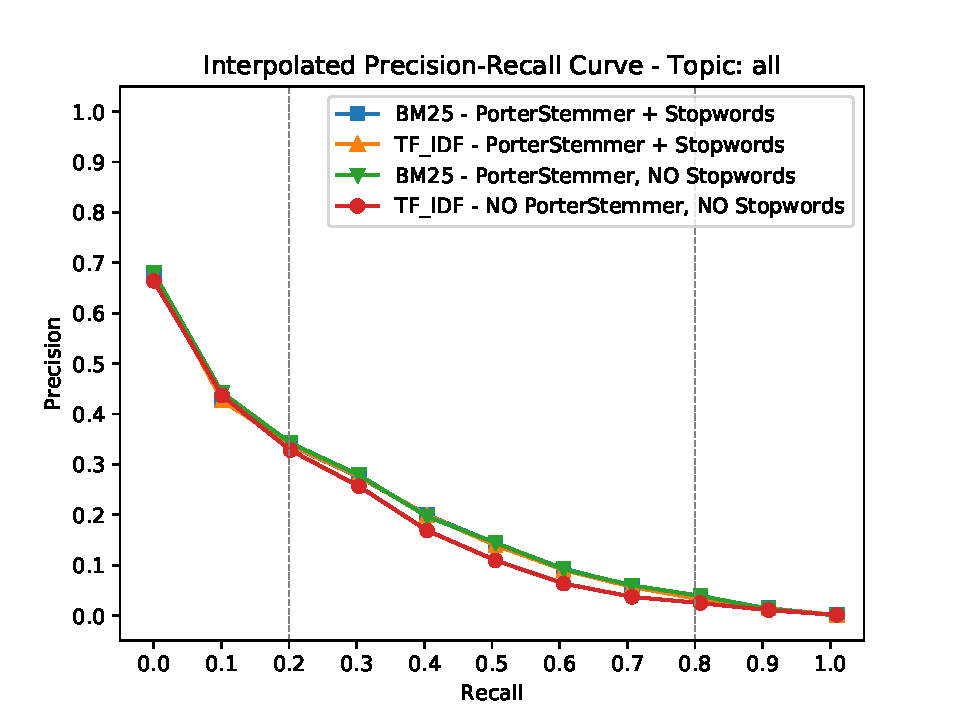
\includegraphics[scale=0.55]{figures/iprc.pdf}
    
    \caption{Valori (interpolati) medi sui 50 topic di \textit{precision} a diversi livelli di \textit{recall}. L'andamento della curva è prevedibile in quanto al crescere del numero di documenti reperiti aumenta anche il numero di documenti non rilevanti reperiti, facendo così diminuire la \textit{precision} \cite{measures}. Le linee veritcali grigie facilitano il confronto fra i sistemi delimitando le tre aree in cui risulta essere più interessante compararli \cite{measures}. Nessun sistema sembra essere notevolmente migliore rispetto agli altri.}
    \label{fig:iprc}
\end{figure}


\subsection{Hypothesis Testing}
I risultati ottenuti in fase di evaluation non sono sufficienti a determinare quale modello sia significativamente il migliore; per provare a fare ciò è necessario ricorrere a dei test statistici. Usiamo one-way ANOVA (Tabella \ref{tab:anova}) per determinare se almeno uno dei sistemi risulti essere significativamente diverso dagli altri, successivamente, per individuare tale sistema (o sistemi), facciamo un confronto \textit{pairwise} fra di essi attraverso il test di Tukey (Figura \ref{fig:tukey_maps}).

\begin{table}[h]
\centering
\begin{tabular}{|l|r|r|}
\hline
\textbf{Measure} & \textbf{F-stat} & \textbf{p-value} \\ \hline
MAP              & 0.0997          & 0.9601           \\
RPrec            & 0.0567          & 0.9822           \\ 
P@10             & 0.0446          & 0.9875           \\
\hline
\end{tabular}
\caption{I valori della colonna \textit{p-value} indicano la probabilità di osservare misure simili in presenza dell'ipotesi nulla. Essendo alti non abbiamo prove empiriche per rigettare tale ipotesi, la quale sostiene che le misure ottenute nei 50 topic dai 4 sistemi provengono dalla stessa distribuzione di probabilità, in breve: nessuno dei sistemi è signficativamente diverso dagli altri (a livello di signficatività 0.05).}
\label{tab:anova}
\end{table}

\begin{figure}[h!]
    \centering
    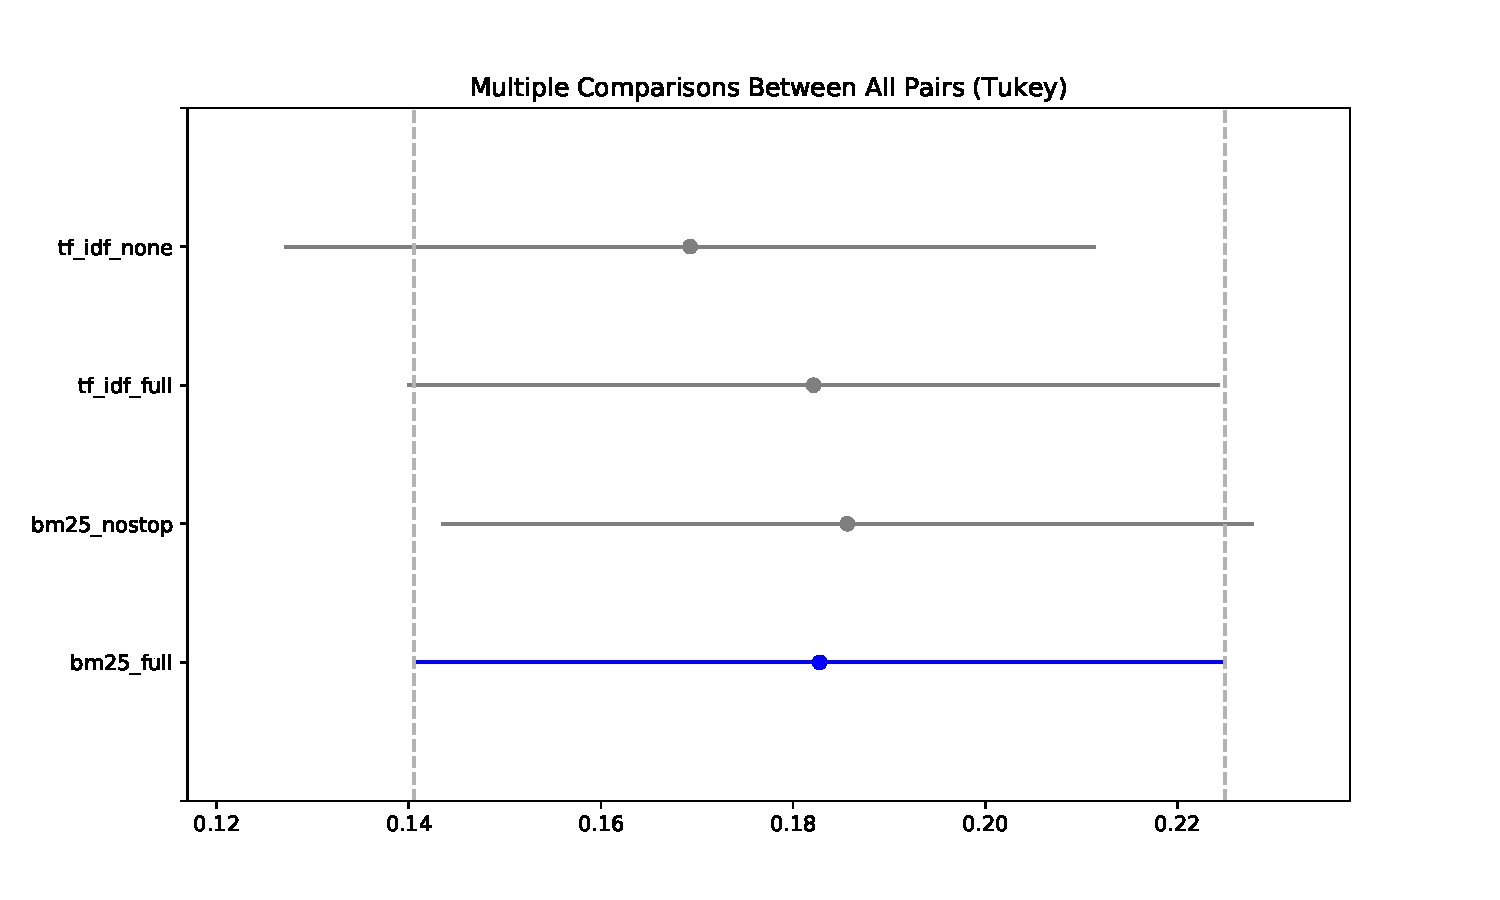
\includegraphics[scale=0.4]{figures/tukey_maps.pdf}
    
    \caption{In blu è colorato l'intervallo di confidenza del sistema che pensavo raggiungesse le migliori performance (\texttt{bm25\_full}); in grigio sono colorati i sistemi NON significativamente diversi dal sistema blu; in rosso (nessuno in figura) sono colorati i sistemi significativamente diversi, ovvero quelli con intervalli di confidenza disgiunti dal sistema blu.}
    \label{fig:tukey_maps}
\end{figure}

\section{CONCLUSIONS}
\todo{Cocnlusioni}
A conclusion section is not required. Although a conclusion may review the main points of the paper, do not replicate the abstract as the conclusion. A conclusion might elaborate on the importance of the work or suggest applications and extensions. 

\addtolength{\textheight}{-12cm}   % This command serves to balance the column lengths
                                  % on the last page of the document manually. It shortens
                                  % the textheight of the last page by a suitable amount.
                                  % This command does not take effect until the next page
                                  % so it should come on the page before the last. Make
                                  % sure that you do not shorten the textheight too much.

%%%%%%%%%%%%%%%%%%%%%%%%%%%%%%%%%%%%%%%%%%%%%%%%%%%%%%%%%%%%%%%%%%%%%%%%%%%%%%%%



%%%%%%%%%%%%%%%%%%%%%%%%%%%%%%%%%%%%%%%%%%%%%%%%%%%%%%%%%%%%%%%%%%%%%%%%%%%%%%%%



%%%%%%%%%%%%%%%%%%%%%%%%%%%%%%%%%%%%%%%%%%%%%%%%%%%%%%%%%%%%%%%%%%%%%%%%%%%%%%%%
\begin{thebibliography}{99}
\bibitem{scipy} Jones E, Oliphant E, Peterson P, et al. SciPy: Open Source Scientific Tools for Python, 2001, http://www.scipy.org/ 
\bibitem{statsmodels} Seabold, Skipper, and Josef Perktold. “Statsmodels: Econometric and statistical modeling with python.” Proceedings of the 9th Python in Science Conference. 2010.
\bibitem{measures} \texttt{https://trec.nist.gov/pubs/trec16/appendices/measures.pdf}
\todo{add lulz}
\end{thebibliography}
\end{document}
